\documentclass[notitlepage,groupedaddress]{IEEEtran}
%\documentclass{revtex4-1}
\usepackage{graphicx}
\usepackage{morefloats}
\usepackage{placeins}
\usepackage{supertabular}
\usepackage{amsmath, amsthm, amssymb}
\usepackage{hyperref}
\usepackage{array}
\usepackage{subfig}
\usepackage{listings}
\usepackage{multirow}
\usepackage{booktabs}
%\pdfminorversion=4
\usepackage[font=small]{caption}
\hypersetup{colorlinks, linkcolor=blue,citecolor=blue, urlcolor=blue}
\newcommand{\ACK}{\emph{ACK}}
\makeatletter
\def\verbatim{\small\@verbatim \frenchspacing\@vobeyspaces \@xverbatim} 
\makeatother
%\usepackage{cite}

% Default fixed font does not support bold face
\DeclareFixedFont{\ttb}{T1}{txtt}{bx}{n}{12} % for bold
\DeclareFixedFont{\ttm}{T1}{txtt}{m}{n}{12}  % for normal
\usepackage{color}
\definecolor{deepblue}{rgb}{0,0,0.5}
\definecolor{deepred}{rgb}{0.6,0,0}
\definecolor{deepgreen}{rgb}{0,0.5,0}
\newcommand{\fix}[1]{\texttt{\small #1}}
\newcommand{\sfix}[1]{\texttt{\scriptsize #1}}
\newcommand{\code}[1]{\texttt{\small #1}}

 

%\newcommand{\code}[2]{
%  \hrulefill
%  \subsection*{#1}
%  \lstinputlisting{#2}
%  \vspace{2em}
%}

\begin{document}
\title{ECE542 Final Report\\ Computing Reliability of IlliniSat}
\author{Eric Badger (badger1), Zachary Estrada (zestrad2), Matthew Tischer
(tischer1)}
%FIXME: Write your names, group name, data range in your dataset and the
%data-set assigned to you on the report.

\maketitle
%\begin{abstract}
%\end{abstract}


%\nocite{*}

\section{Project Statement}\label{sec:problem}

A CubeSat is a small satellite ($\sim$~1kg) constructed out of (usually)
commodity components that is used for scientific research or educational
purposes.  The University of Illinois has a
CubeSat\footnote{\url{http://cubesat.ae.illinois.edu/index.php}} program in
which a class and dedicated team have been developing a scalable picosatellite
bus, IlliniSat-2 (hereafter referred to as ``IlliniSat.''  IlliniSat is intended
to be used for multiple missions, the first of which (Lower
Atmosphere/Ionosphere Coupling Experiment, LAICE) is planned to launch around
December 2014.  This mission will involve three scientific payloads: one from
Illinois and two from Virginia Tech.  In collaboration with Bindu Jagannatha and
Alex Ghosh of the IlliniSat team, this project aims to analyze and enhance the
reliability of the computing systems used in IlliniSat.

The IlliniSat bus contains various systems, and this project focuses on the
Command and Data Handling (C\&DH) system.  The C\&DH system is responsible for
maintaining the mission schedule and coordinating the communication of the
satellite with the ground station.  It also interacts with other systems, such
as the Attitude Determination and Control System (ADCS), which is responsible
for maintaining proper orientation of the satellite. A state diagram for
IlliniSat, provided by the IlliniSat team, is shown in Figure
\ref{fig:state_machine}. The C\&DH system is based on a MitySOM-335x Processor
Card, built with a TI AM335x Application Processor System-on-Chip
(SoC).\footnote{\url{http://www.criticallink.com/wp-content/uploads/MitySOM-335x_Datasheet.pdf}}
An embedded Linux distribution, Arago, is run on top of the TI SoC and
IlliniSat's functionality is implemented in set of userspace daemons. The
standard \fix{atd} utility (modified for the IlliniSat platform) is used to
schedule tasks.

%FIXME: increase font size?
\begin{figure}
  \centering
  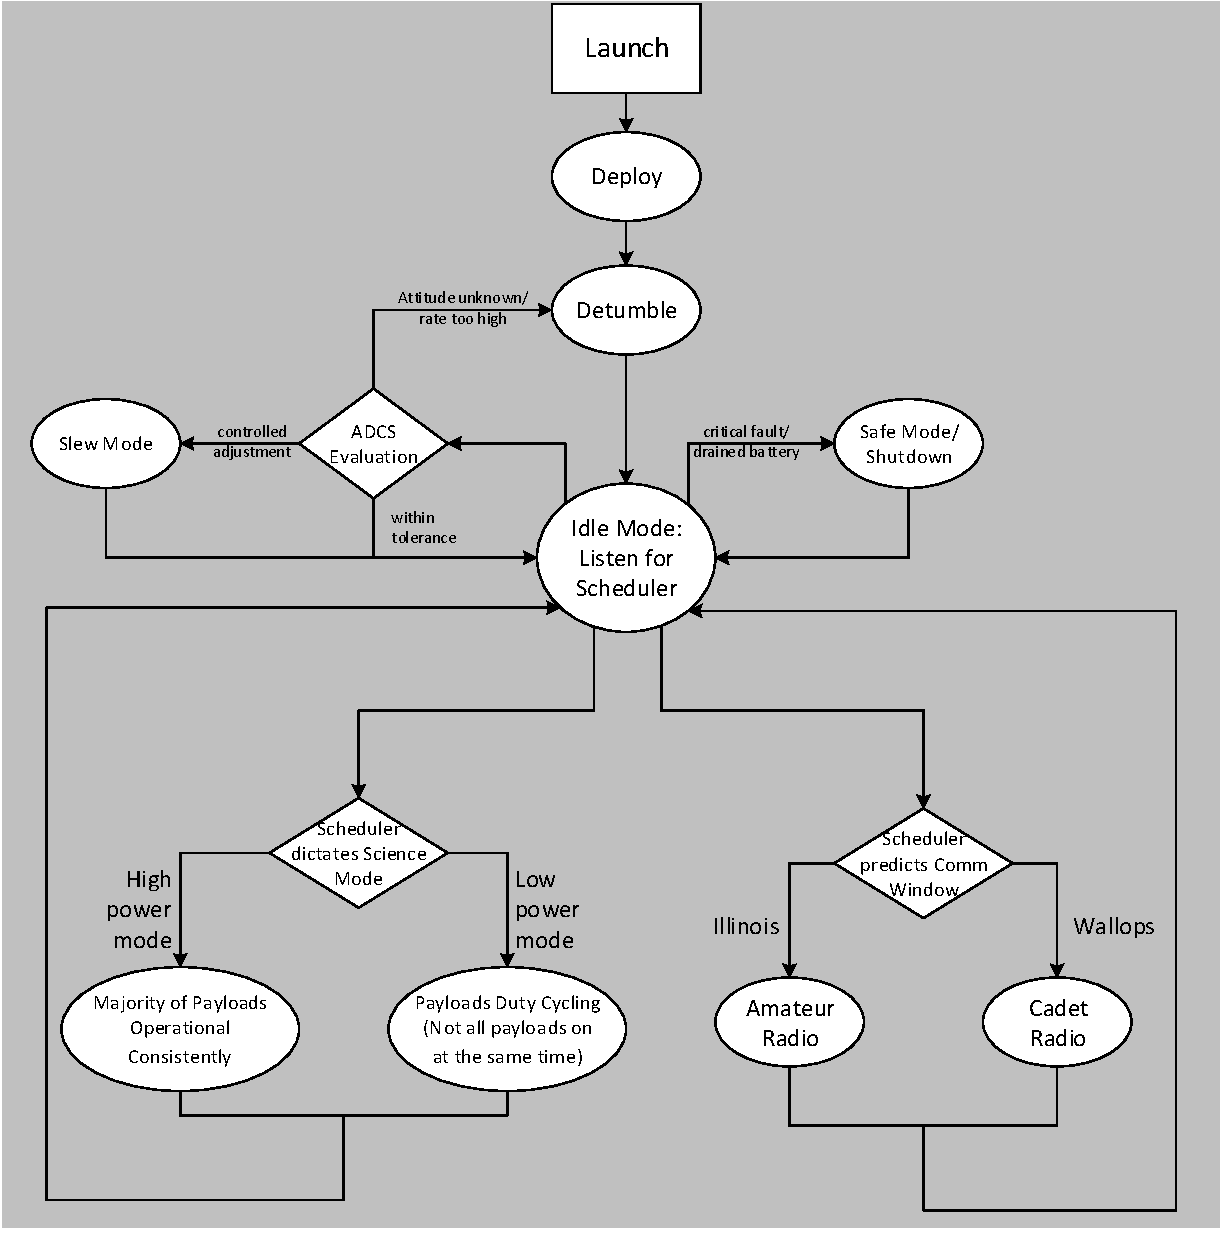
\includegraphics[width=0.5\textwidth]{images/state_machine}
  \caption{The main function of the C\&DH system is to operate the satellite
  through this state diagram. After \textbf{launch} and \textbf{deploy}, the
  system starts in the \textbf{detumble} state (which can also be reentered in
  an emergency situation): it calculates its attitude and points to the sun to
  charge the battery.  \textbf{Idle:} this is the mode where the satellite works
  through its mission schedule and ensures it has the proper attitude for data
  collection, the system can remain in this state to charge its battery.
  \textbf{Science modes:} this is the normal operating mode of the satellite
  where the C\&DH subsystem collects data, and if there is not enough power it
  will only run a subset of the experiments.  \textbf{Communication modes:} this
  is when a radio is active and communicating with a ground station.
  \textbf{Slew mode:} C\&DH relinquishes control to the ADCS when it detects
  that the satellite may need repositioning.  \textbf{Safe mode:} low-power
  default mode when a fault is detected, the satellite will broadcast an error
  code to the ground station.  \textbf{Shutdown:} all non-crucial systems are
  shutdown when battery power is critically low. Figure courtesy Alex Ghosh and
  Bindu Jagannatha. }\label{fig:state_machine}
  %FIXME: finish writing this
\end{figure}

Currently, the system has a watchdog timer that will reboot the flight computer
if it does not receive a heartbeat every 60 seconds.  The watchdog is part of a
health monitoring system that also observes the state of the battery, satellite
attitude, temperature, etc. If the health monitor determines that the system is
in a faulty state, it will transition C\&DH into a recovery mode (e.g. if the
battery is low, switch off all nonessentials and point the satellite towards the
sun).
%FIXME: do we want the health monitor figure?
%FIXME: define SPoF

\subsection{Design Constraints}
The IlliniSat bus has many hardware and software requirements that constrain our
improvements of the system. Since the IlliniSat team has already chosen their
hardware, we will have to make all of our changes in software. Given the nature
of the mission, the software is required to have mission critical components
that cannot fail. The main design constraints that will be put on us while
improving the system are the following:
\begin{itemize}
  \item Preserve real-time deadlines
  \item Minimize additional power consumption
  \item Avoid complex solutions
\end{itemize}
IlliniSat needs to be constantly reacting to its environment so that it can
interface with payloads, communicate to the ground, and monitor the health of
the system, among other things. Because of this, hard real-time deadlines are
required and cannot be missed. 

Since IlliniSat is such a small satellite with stringent physical dimensions and
therefore limited battery capacity, power is a major concern for the team.  If
too much power is consumed, the battery may not last while the satellite is not
receiving solar power (if it is either eclipsed by the earth or positioned
poorly).  Also, if the system is charging and the CPU is loaded, components may
start to overheat.  Any software reliability techniques used should therefore be
mindful not to use too much power and should also be aware of the current state
of the satellite (recovery modes, etc...).

Finally, the IlliniSat team has requested that we keep our solution simple (and
well documented) so that it can be implemented and maintained easily.
Furthermore, we need to be careful not to implement overly intricate solutions
that may introduce new failure modes or reduce the system's reliability.

\section{Related Work}\label{sec:related_work}
There is already an existing body of work that deals with small satellites and
investigations of their reliability.  In \cite{odegaard2013error}, the author
discusses developing software systems to increase the reliability of a small satellite.
The use of a recovery mode, one of the systems discussed in
\cite{odegaard2013error}, is already present in IlliniSat.
\cite{odegaard2013error} also proposes solutions for protecting the satellite's
program code, although its implementation is unable to handle the case of a
corrupted kernel with no saved system checkpoints; our proposed approach stores
multiple copies of the kernel, so it is able to recover even if the kernel image
is completely corrupted.

There has also been significant work in using hardware-based reliability measures in small satellite designs.  \cite{toorian2008cubesat} mentions redundancy and watchdog timers as two solutions to ensure CubeSat reliability.  In \cite{passerone2008design}, the authors partially provide reliability in their satellite by using five fully redundant processors.   As the IlliniSat project has already fixed its hardware requirements and as we wish to produce advice and solutions that can be directly applied to IlliniSat, we do not consider these approaches in this work.

Looking into commercial CubeSat implementations, we were not able to 
find any apparent software reliability solutions in their systems.\footnote{\url{http://www.clyde-space.com/cubesat_shop/software}}$^\textnormal{,}$\footnote{\url{http://www.isispace.nl/cms/index.php/products-and-services/missions}}$^\textnormal{,}$\footnote{\url{http://www.gomspace.com/index.php?p=products-software}}
The suppliers mentions that their system is reliable, but this is because
they are flight tested, not because of any software reliability techniques that
have been employed.  We also investigated other university systems, but our
search did not reveal any relevant information on their CubeSat websites.

However, the commercial suppliers do offer hardware solutions. Most commonly
the hardware is radiation-hardened to lessen the likelihood of transient cosmic ray
failures in space.\footnote{\url{http://www.spacemicro.com/space-components.html}}$^\textnormal{,}$\footnote{\url{http://www.aacmicrotec.com/images/Products/Components/MCC_website.pdf}}





\section{Approach}\label{sec:approach}

\section{Work Distribution}\label{sec:team}
Throughout the course of this project, we maintained open communication and met
regularly.  Since we started off with three separate objectives, it became clear
that it would be best to split off into multiple directions.  The original plan
was to split into these multiple directions and converge on whichever solution
seemed most feasible, in anticipation of some subprojects failing.  However,
this did not happen so we accomplished all that we started to do.  The final
work distribution ended up being:\\

\noindent Matt
\begin{itemize}
  \item{Fault model development}
  \item{M\"obius simulation}
\end{itemize} 
\noindent Zak
\begin{itemize}
  \item{Boot protection modifications for U-boot}
  \item{Fault injection for U-boot and daemons}
\end{itemize}
\noindent Eric
\begin{itemize}
  \item{Flash patrol daemon}
  \item{CRC checker daemon}
\end{itemize}

\section{Results}\label{sec:results}

\subsection{M\"obius Results}\label{sec:mobiusresults}

One surprising result of this simulation involved the \texttt{num\_replicas} parameter, which controlled the number of copies of the operating system image saved on an individual device.  When we first ran this simulation, we believed that our model was incorrect because the system reliability was completely unaffected by the \texttt{num\_replicas} parameter.  In order to further debug the system, we added additional places to the model to keep track of the number of SEU and SEFI events that were recorded in the system.  To our surprise, M\"obius reported that an average of 0.0 SEU events (with 95\% confidence interval width 0.0) occured over 1000 simulation runs; as M\"obius reports small numbers that it can detect, this average likely indicates that no SEU occured during each of the 1000 simulations.  In retrospect, this conclusion is reasonable; the SEU error rate is on the order of $10^{-7}$ events per day, which corresponds to an average time before failure of over 27,000 years.  In addition, an SEU only corrupts a kernel if it modifies any of the data in that kernel.  We assumed that each kernel took up 10MB of space and that errors were uniformly distributed across the 512MB flash chip.  As a result, any SEU that occurred had a $\frac{10\cdot\textrm{number of kernels}}{512}$ chance of actually corrupting a kernel.  These two factors combined indicated that the probability of an SEU affecting a kernel on the given Micron flash memory was essentially zero.

As the probability of an SEU event in this model affecting a kernel was essentially zero, we recognized that controlling SEFI events was the key toward maintaining reliable operation.  In order to accomplish this goal, we expanded our model to include $n$ independent devices, each containing $m$ copies of the kernel.  Each device has its own controller hardware and fails independently, so the system is able to handle $n-1$ SEFIs without failing.  We also focused on testing the periodic reboot parameter discussed in Section \ref{sec:buildingmodel}.

The results of this simulation are shown in Figure \ref{fig:reliability} and Table \ref{tab:reliability}.  The 95\% confidence interval width is plotted for each point in Figure \ref{fig:reliability} and is also included in Table \ref{tab:reliability}

\begin{figure}[width = 0.5\textwidth]
\centering
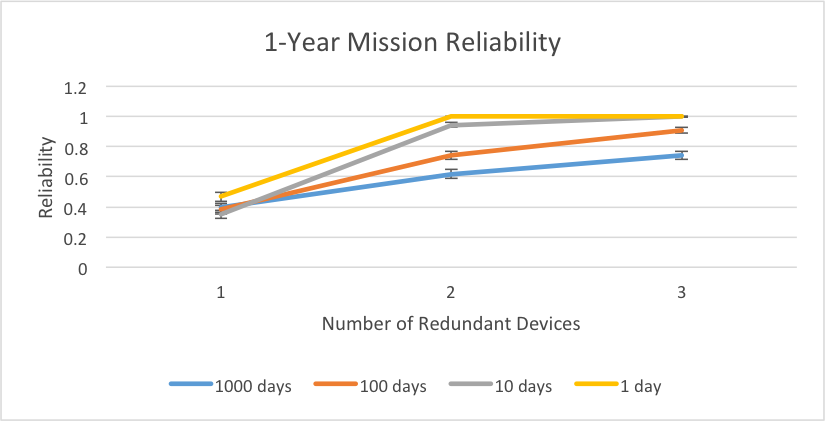
\includegraphics[scale=0.6]{reliability}
\caption{1-year mission reliability calculated in  our model}\label{fig:reliability}
\end{figure}

\begin{table}[width = 0.5\textwidth]
{\scriptsize
\centering
\begin{tabular}{ccccc}
\toprule
& \multicolumn{4}{c}{\bf Flash Reboot Interval (days)}\\
\cmidrule(r){2-5}
{\bf \#Dev} & 1000 & 100 & 10 & 1\\
\midrule
1 & 0.395 $\pm$ 0.030 & 0.383 $\pm$ 0.030 & 0.351 $\pm$ 0.030 & 0.468 $\pm$ 0.031 \\
2 & 0.618 $\pm$ 0.030 & 0.741 $\pm$ 0.028 & 0.944 $\pm$ 0.014 & 0.998 $\pm$ 0.001 \\
3 & 0.740 $\pm$ 0.027 & 0.908 $\pm$ 0.018 & 0.998 $\pm$ 0.003 & 1.000 $\pm$ 0.000 \\
\bottomrule
\end{tabular}
\caption{1-year mission reliability for our model}\label{tab:reliability}
}
\end{table}

As the graphs indicate, the default reliability of the IlliniSat system is fairly low; there is approximately a 40\% chance that the satellite will survive a year under this model.  However, the introduction of another device improves reliability slightly.  If at least two devices are available, periodically power-cycling the flash memory provides an additional, significant reliability improvement.  If the flash is power cycled daily, we are able to achieve an estimated reliability of 99.8\%, a significant improvement over our initial condition.

\subsection{Fault Injection Tool}

In order to test the utilities developed, we built a small fault injection
tool.  Since both the boot protection and flash patrol daemon interact with
storage in some form, one tool was made for testing both utilities.  The tool
opens a file ands seeks to a specified location (usually chosen uniformly at
random) and then reads a bit, flips it, and writes it back.  When writing
directly to block devices, the {\texttt {O\_DIRECT}} flag is used to ensure
writes are flushed immediately.

%FI MERGE ANCHOR
\subsection{Boot Protection}
To evaluate the boot protection scheme, we flipped a bit in the region of the
QEMU virtual flash device used to hold the boot protection script and the kernel
images.  This experiment was then repeated by uniformly flipping bits at random
in this region.  Of the 610 boot attempts made during the injection campaign,
602 were successful.  This corresponds to a recovery rate of 98.4\%, and we note
that this recovery rate is for failures inside the boot region, not across the
entire device (512MB in the case of IlliniSat).  When examining the output, 214
boots had CRC errors in the first kernel, which matches expectations as there
were three copies of the kernel (considering that there are three copies of the
kernel in the flash image, this matches expectations).  We leave targeted
injections against the protection script for future work.

%BP MERGE ANCHOR
\subsection{Flash Patrol Daemon}
%TODO: wonder what would happen if we bind mounted the directory and injected
%into that...
The flash patrol daemon monitors a Linux filesystem.  However, since the
inotify subsystem sends events based on file updates, we cannot simply
inject into the files in the directory being watched by inotify (as this would
force a CRC update). Therefore, we use our fault injection utility to inject
into the actual block device (e.g.  \texttt{/dev/sdb1}).  The files in the
filesystem are sample data files provided from the IlliniSat team and copied
until the filesystem is full (for the speed of experiments, we use a 7.5MB disk
partition).  At each experiment, we need to start with a clean slate, so we
regenerate the filesystem and recopy over the data.  After that, we flip a
random bit inside the underlying block device and record whether the daemon can
detect a failure.  We performed 402 such experiments and detected 337 errors,
corresponding to 83.8\% of injections resulting in a detected CRC error.
Note that faults were injected into non-data regions of the filesystem, so the
detection rate is likely much higher than 83.3\%.
%TODO: kill patrold and just run simple checkerd experiments?

\section{Project Insights}\label{sec:insights}

This study has also shown that a solution to the boot reliability problem need not be costly in terms of either time or effort.  Two flash storage devices are enough to provide for kernel integrity, and many off-the-shelf devices provide support for an extra storage device.  Power cycling flash memory on a daily basis is enough to provide almost three 9s of reliability and should only require a few minutes per day to perform the power cycle.

\subsection{Further Recommendations}
Based on other observations during this project and past experience, we would
like to make the following recommendations to the IlliniSat team.

\subsubsection{Reboot on panic} By default, when the Linux kernel fails, it
issues a ``kernel panic'' message and halts the system.  While IlliniSat's
watchdog should detect this scenario, the kernel has the ability to
automatically reboot on panic.  Enabling this can help ensure the system will
reboot in the event of a transient kernel error. The system will either reboot
faster than waiting for a watchdog timeout since the kernel will issue the
reboot almost immediately after failure or it will still reboot in the unlikely
event of a watchdog failure.

\subsubsection{OOM-killer} The Linux kernel that the IlliniSat team is using
has an Out-Of-Memory killer (OOM-killer) built into it. When the system is 
low on main memory, the OOM-killer will kill a process based on some heuristics.
However, this can have undesirable consequences if it kills certain processes.
We recommend that IlliniSat either be mindful of this and tune the OOM-killer
such that processes are killed in an acceptable order or that the kernel be set
to panic on OOM~\cite{oracleoom}.

%OOM Merge anchor
\subsubsection{Regular Reboot} Our results from the M\"obius simulation model
in Table \ref{tab:reliability} support a regular reboot of the system. For a one year
mission, 1000 days without reboot is effectively the same as never rebooting. The
difference between this and rebooting every day for 2 and 3 devices increases the
reliability from 0.618 to 0.998 and 0.740 to 1.000 respectively. This is a change in
38\% and 26\% respectively which is a very large increase in system reliability. 
Even in the case of a single device, the reliability increases by 7.3\% from 39.5\%
to 46.8\% Because of the increase in reliability with little to no additional overhead, 
we urge the team to force regular reboots of the system every day.

\section{Project Impact}\label{sec:impact}

\section{Future Work}\label{sec:future_work}
\begin{itemize}
  \item Consider adding MityARM335x to QEMU
  \item {\bf Model different hardware.}  While the M\"obius simulation used in this experiment was tuned to the board being used by the IlliniSat team, CubeSat is designed to be used on low-cost commodity hardware.  Studies such as \cite{Oldham2008TID} found a four-order-of-magnitude difference in flash memories of the same size from different manufacturers.  Our solution to the boot protection problem was designed to minimize the effects of SEFI failures because the IlliniSat hardware has a relatively high SEFI rate; we would most likely recommend different strategies for memories where the risk of SEU is non-negligable and the risk of SEFI is less significant.
  \item {\bf Model longer mission lifetimes.}  One of the major assumptions that guided the development of our fault model was the assumption that the IlliniSat mission had at most a 1 year lifetime.  This assumption simplified the model because the Total Ionizing Dose (TID) that the satellite received was small enough to have no effect during the course of the mission \cite{Likar2010Novel, Oldham2008TID}.  However, TID-related failure is a significant failure mode that could occur during longer missions.  By extending the model to support larger mission lifetimes, we would be able to better characterize reliability challenges for long-term CubeSat missions.
  \item {\bf Provide additional software assurance.} While this project primarily focused on providing fault-tolerance from hardware errors via software, we believe that a formal analysis of the IlliniSat software stack would also help to provide dependability.  As our failure model only considers operating system level failures, it is unable to protect against application-level crashes or errors that could exist in the IlliniSat software.  We chose not to work on this topic for our project because the software is currently being developed; however, we could certainly revisit it in the future.
\end{itemize}


%\section*{acknowledgments}

\bibliographystyle{IEEEtran}
\bibliography{final_report}

%\clearpage
%\onecolumn
%\section{Code}
%\lstset{
%  language=Python,
%  showstringspaces=false,
%  formfeed=\newpage,
%  tabsize=2,
%  commentstyle=\itshape,
%  basicstyle=\ttfamily,
%  morekeywords={models, lambda, forms},
%  %basicstyle=\ttm,
%  %keywordstyle=\ttb\color{deepblue},
%  %otherkeywords={self},             % Add keywords here
%  %emph={Event,__init__},          % Custom highlighting
%  %emphstyle=\ttb\color{deepred},    % Custom highlighting style
%  %stringstyle=\color{deepgreen},
%}
\end{document}
